\documentclass[10pt,a4paper]{article}

\newcommand{\COLORSDIR}{/Users/hoolywear/Desktop/UNIMORE/II ANNO/II SEMESTRE/colors}

\usepackage[italian]{babel}
\usepackage[usenames,dvipsnames,table]{xcolor}
\usepackage[utf8]{inputenc}
\usepackage[T1]{fontenc}
\usepackage{soul}
\usepackage[a4paper, portrait, margin=2.5cm]{geometry}
\usepackage{array}
\usepackage{tabularx}
\usepackage{multicol}
\usepackage{amsmath}
\usepackage{amsfonts}
\usepackage{amssymb}
\usepackage{algorithmicx}
\usepackage[noend]{algpseudocode}
\usepackage{wrapfig}
\usepackage{graphicx}
\usepackage{hyperref}
\hypersetup{
    colorlinks=true,
    linkcolor=black,
    filecolor=magenta,      
    urlcolor=cyan,
    pdftitle={Overleaf Example},
    pdfpagemode=FullScreen,
    }
\urlstyle{same}
\usepackage{caption}
\usepackage{capt-of}
\captionsetup[figure]{name=Fig.}
\renewcommand{\thefigure}{\arabic{section}.\arabic{figure}}
\graphicspath{ {./images/} }

\input{\COLORSDIR/colors_4}

\usepackage{listings}

\definecolor{codeblue}{HTML}{1e66f5}
\definecolor{codepurple}{HTML}{8839ef}
\definecolor{codered}{HTML}{d20f39}
\definecolor{darkbluenord}{HTML}{232731}
\definecolor{lightbluenord}{HTML}{b1bfe3}

\lstdefinestyle{code}{
    backgroundcolor=\color{gray!10},   
    basicstyle=\ttfamily,
    commentstyle=\color{codeblue},
    keywordstyle=\color{codered},
    breakatwhitespace=false,         
    breaklines=true,                 
    captionpos=b,                    
    keepspaces=true,                 
    showspaces=false,                
    showstringspaces=false,
    showtabs=false,                  
    tabsize=2,
    mathescape=true %dollar signs act as inline math delimiters
}

\lstdefinestyle{python}{
    style=code,
    language=python,
    commentstyle=\color{codeblue},
    keywordstyle=\color{codepurple},
    stringstyle=\color{codered}
}

\lstset{style=code,language=C++}

\usepackage[framemethod=TikZ]{mdframed}

\mdfsetup{%
  roundcorner=8pt}

% styles
\def\Clinewidth{.8pt}
\mdfdefinestyle{titlerule}{%
  frametitlerule=true,%
  frametitlerulewidth=\Clinewidth,%
  subtitleaboveline=true,subtitlebelowline=true,%
  subtitleabovelinewidth=\Clinewidth,subtitlebelowlinewidth=\Clinewidth,%
linewidth=1pt}

\mdfdefinestyle{emphasize}{%
  style=titlerule,%
  frametitle=,%
  linecolor=gray!50,linewidth=1pt,backgroundcolor=gray!10}

% algorithmic environment
\surroundwithmdframed[backgroundcolor=gray!10,hidealllines=true,%
frametitle={}]{algorithmic}

% quote environment
\surroundwithmdframed[style=emphasize]{quote}

% example environment
\newmdenv[frametitle=Esempio,style=titlerule]{example}

% emphasize environment
\newmdenv[style=emphasize,%
          linecolor=emp!70!red,backgroundcolor=emp]{emphasize}

% blue emphasize environment
\newmdenv[style=emphasize,%
          linecolor=obs!70,backgroundcolor=obs!20]{emphasize-blue}

%% NOT USED IN III ANNO
%% % definition environment
%% \newmdenv[frametitle=Definizione,style=titlerule,%
%%           linecolor=def]{definition}
%% 
%% % theorem environment
%% \newmdenv[frametitle=Teorema,style=titlerule,%
%%           linecolor=the]{theorem}
%% % observation environment
%% \newmdenv[frametitle=Osservazione,%
%%           backgroundcolor=white,linecolor=obs,%
%%           frametitlebackgroundcolor=obs]{observation}
%% 
%% % warning environment
%% \newmdenv[style=emphasize,%
%%           backgroundcolor=war!10,linecolor=war]{warning}

\author{Iacopo Ruzzier}
\date{Ultimo aggiornamento: \today}


\title{%
Compilatori\\
\large Parte Due}

\begin{document}
\maketitle
\tableofcontents
\newpage
\section{Introduzione (25 feb)}

\subsection{Motivazione}

Ricordiamo il ruolo del compilatore tra le tecnologie informatiche, quello dell'ISA e del linguaggio assembly, i passaggi gestiti dal compilatore, dall'assembler, eccetera
\begin{itemize}
  \item Il compilatore \textbf{traduce un programma sorgente in linguaggio macchina}
  \item L'ISA agisce da "interfaccia" tra HW e SW (fornisce a SW il set di istruzioni, e specifica a HW che cosa fanno)
\end{itemize}

\subsubsection{La funzione dei compilatori}

\begin{itemize}
  \item Funzione principale e pi\`u nota: trasformare il codice \textbf{da un linguaggio ad un altro} (es. C $\rightarrow$ Assembly RISC-V) (ricordiamo che \`e solo il primo passo di un'intera toolchain di programmi per creare eseguibili)

\item Gestendo la traduzione a linguaggio macchina al posto dei programmatori, l'altra funzione importante \`e l'\textbf{ottimizzazione} del codice, che permette la \textbf{produzione di eseguibili di stesse funzionalit\`a}, ma diversi a livello di \textbf{dimensioni} (es. per sistemi embedded e high-performance), \textbf{consumo energetico}, \textbf{velocit\`a di esecuzione}, ma anche in termini di determinate \textbf{caratteristiche architetturali} utilizzate (es. proc.~multicore)
\end{itemize}

\subsubsection{L'evoluzione dei compilatori}

Le rivoluzioni in termini di "classe" di dispositivi e di dimensioni dei transistor sono molto frequenti (Bell, Moore), e nei primi 2000 si arriva ai \textbf{limiti fisici della miniaturizzazione e della frequenza} operativa dei processori (e conseguenti problemi di dissipazione del calore prodotto) $\rightarrow$ nasce l'idea di cambiare completamente il paradigma di sviluppo di un processore: dal singolo core sempre pi\`u potente passo a \textbf{pi\`u core "isopotenti"} sullo stesso chip

\noindent\begin{minipage}[c]{.3\textwidth}
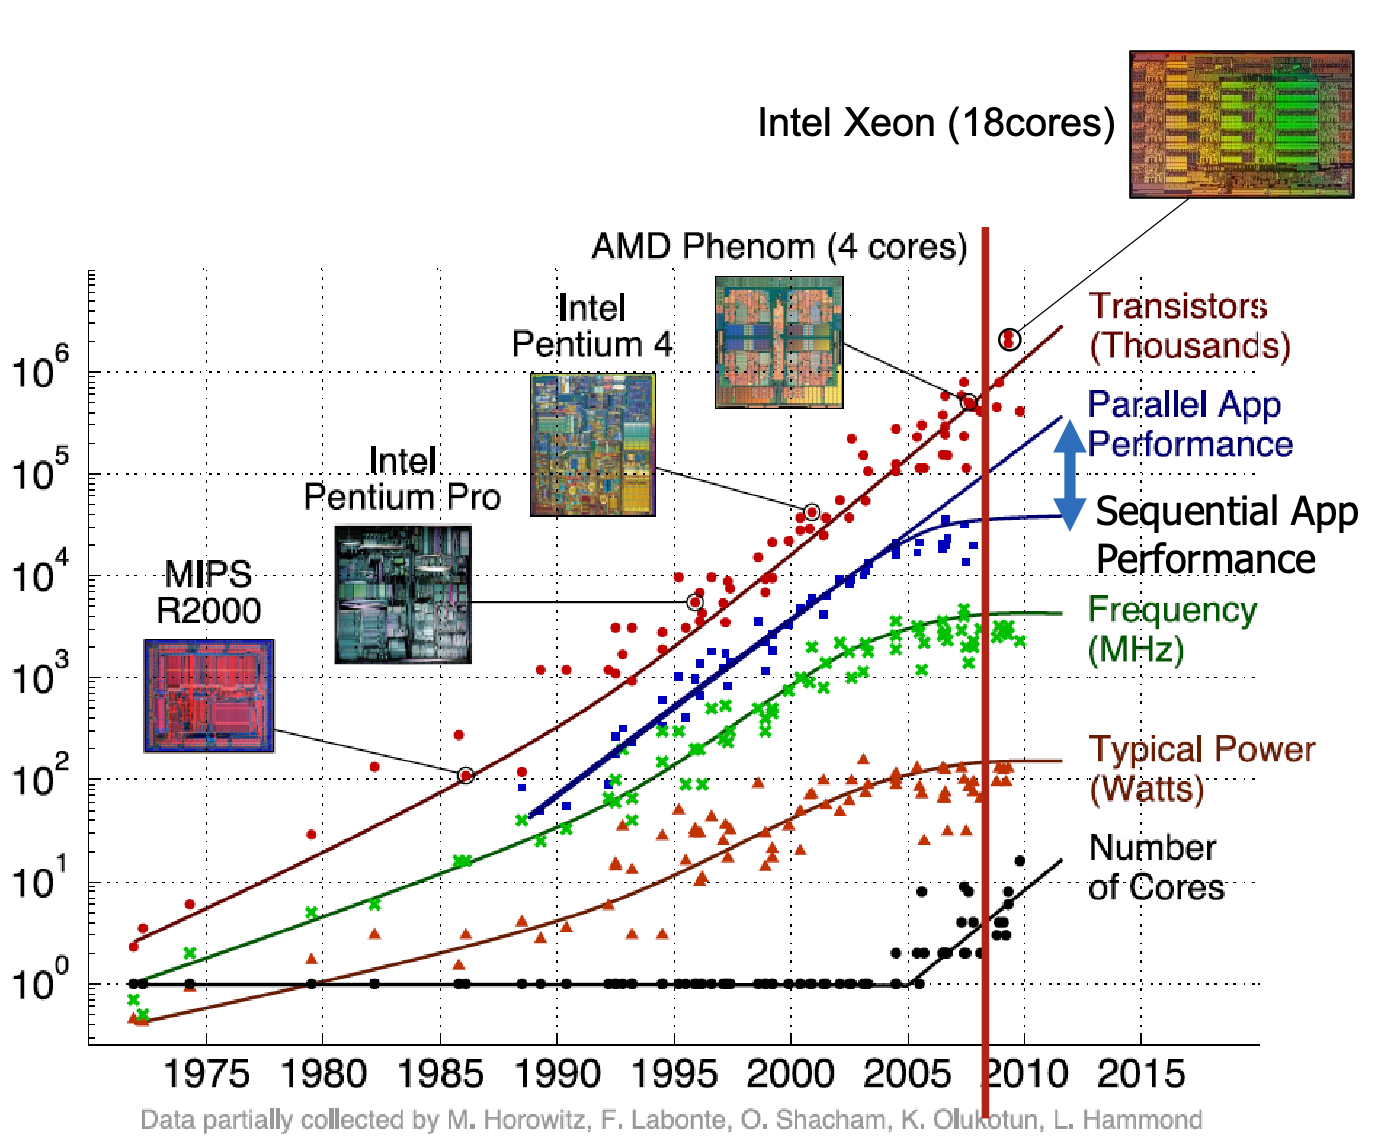
\includegraphics[width=\textwidth]{intro_1.png}
\end{minipage}
\begin{minipage}[c]{.7\textwidth}
  Notiamo come dal 2005 circa si raggiunge un plateau in termini di consumo, di frequenza e di performance di programmi \textit{sequenziali}, e aumenta la performance di programmi che \textbf{sfruttano la parallelizzazione} $\rightarrow$ i programmi devono essere "consapevoli" che il processore \`e multicore! Qui capiamo l'impatto dello sviluppo tecnologico sull'evoluzione dei compilatori
\end{minipage}

\begin{emphasize}
  Per evitare un cambio nella formazione dei programmatori, le aziende sperano nei compilatori autoparallelizzanti - non sar\`a mai possibile e nel mentre sono stati introdotti molti paradigmi di pr.~parallela
\end{emphasize}

Il compilatore mantiene un ruolo fondamentale: oltre a rendere meno "traumatico" il passaggio alla programmazione parallela, si interfaccia con i nuovi paradigmi di programmazione parallela offerti ai programmatori: il programmatore sfrutta interfacce semplici e astratte, mentre il compilatore traduce i costrutti in codice parallelo eseguibile (es. OpenMP)

\subsubsection{Eterogeneit\`a architetturale}

La programmazione parallela e il parallelismo architetturale sono oggi paradigmi consolidati, e i processori general purpose (seppur multicore e ottimizzati) non sono sufficienti per alcune attivit\`a specializzate come la grafica $\rightarrow$ nascono componenti \textbf{acceleratori} di vario tipo: GPU, GPGPU, FPGA, TPU, NPU...
Questo complica ulteriormente la scrittura del software, e dunque impone altre evoluzioni nei compilatori e nelle ottimizzazioni.

\subsection{Ottimizzazione}

Ricordiamo le metriche usate:

\noindent\begin{minipage}[c]{.5\textwidth}
\begin{equation*}
  \text{Performance} = {{1}\over\text{Execution Time}}
\end{equation*}
\end{minipage}
\begin{minipage}[c]{.5\textwidth}
\begin{equation*}
  \text{Execution Time} = {\textcolor{blue}{\text{Instruction Count}} \times \textcolor{red}{\text{CPI}} \over \textcolor{red}{\text{Frequency}}}
\end{equation*}
\end{minipage}\\

Le ottimizzazioni possono avvenire dal punto di vista \textcolor{red}{HW (parametri architetturali)} e da quello \textcolor{blue}{SW (p.~di programma)}. Il compilatore pu\`o agire anche ad es. a livello di cache, aiutando a ridurre i miss e dunque i CPI delle istruzioni \lstinline|load| e \lstinline|store|

\subsubsection{Esempi di ottimizzazione}

\begin{emphasize}
  Distinguiamo le ottimizzazioni che avvengono a compile time o a runtime (statiche o dinamiche)
\end{emphasize}

\begin{itemize}
  \item AS (Algebraic Semplification): ottimizzazione a runtime
  \begin{lstlisting}
-(-i) $\rightarrow$ i
b or true $\rightarrow$ true //cortocircuito logico\end{lstlisting}
  \item CF (Constant Folding):  valutare ed espandere espressioni costanti a compile time
  \begin{lstlisting}
c = 1+3 $\rightarrow$ c = 4
(100<0) $\rightarrow$ false\end{lstlisting}
  
  \item SR (Strength Reduction): sostituisco op. costose con altre pi\`u semplici: classico es. MUL rimpiazzate da ADD/SHIFT (dobbiamo ovviamente tenere conto delle implementazioni hw delle operazioni): esempi a slide 30\\
  esempio sofisticato: for con operazioni su array, sostituito da operazioni su puntatori (aritmetica dei pt.) $\rightarrow$ il risultato si vede nel codice assembly (riporta listings)
\item CSE (Common Subexpression Elimination): elimino i calcoli ridondanti di una stessa espressione riutilizzata in pi\`u istruzioni (statement)
\item DCE (Dead Code Elimination): elimino tutte le istruzioni che producono codice mai letto (e dunque utilizzato), es. variabili assegnate e mai lette, codice irraggiungibile $\rightarrow$ uno dei passi eseguiti pi\`u di frequente durante l'ottimizzazione del codice da parte del compilatore, per rimuovere anche tutto il dead code generato dagli altri passi di ottimizzazione
\item Copy Propagation: per uno statement \lstinline|x = y|, sostituisco gli usi futuri di \lstinline|x| con \lstinline|y| se non sono cambiati nel frattempo (propedeutico alla DCE)
\item CP (Constant Propagation): sostituisco usi futuri di una variabile con assegnato valore costante con la costante stessa (se la variabile non cambia) (slide 38 esempio di sequenza di ottimizzazioni applicate in sequenza) (stiamo sempre ipotizzando che i valori a fine esempi siano poi \textbf{utilizzati}, e non dead code)
\item LICM (Loop Invariant Code Motion): si occupa di muovere fuori dai loop tutto il codice \textbf{loop invariant}; evita i calcoli ridondanti\\
\begin{lstlisting}
while (i<100) {
  *p = x/y + i;
  i = i + 1;
}
\end{lstlisting}
diventa
\begin{lstlisting}
t = x + y;
while (i < 100) {
  *p = t + i;
  i = i + 1;
}
\end{lstlisting}
recupera questione su load e store, questione su CPI medio per una load e quando si riduce/ arriva a 1 (quando si trova in cache, di solito ordine delle decine)\\
chiedi a dani

\end{itemize}

\subsubsection{Ottimizzazioni sui loop}

\begin{itemize}
  \item grande impatto sulla performance dell'intero programma (per ovvie ragioni)
  \item spesso sono ottimizzazioni propedeutiche a quelle machine-specific (effettuate nel backend): register allocation, instruction level parallelism, data parallelism, data-cache locality
  \item sono in generale target delle ottimizzazioni, essendo centrali per il parallelismo
\end{itemize}

\subsection{Anatomia di un compilatore}

Un compilatore svolge almeno due compiti: analisi del sorgente e sintesi di un programma in linguaggio macchina; lo fa operando su una rappresentazione intermedia (IR) che si interpone tra frontend e backend, e tra source code e target code

il blocco di middle-end agisce sul codice intermedio, e in vari passaggi lo trasforma  e lo ottimizza (diverso a seconda del compilatore)

caso llvm: clang (frontend) $\rightarrow$ opt (middleend) $\rightarrow$ llc (backend)

l'ottimizzatore opt si basa su una serie di \textbf{passi di ottimizzazione (o di analisi)}: un passo di analisi scorre l'IR e lo analizza (non lo trasforma, ma produce informazioni utili); un passo di ottimizzazione sfrutta informazioni conosciute per trasformare l'IR (applica le ottimizzazione)


alcune ottimizzazioni non possono essere effettuate o finalizzate senza conoscere l'architettura target (es. sulle cache), e dunque vengono eseguite dal backend

\subsubsection{Flag di ottimizzazione}

sono flag che passo al compilatore (al pass manager) per influenzare \textbf{ordine e numero dei passi di ottimizzazione}
\begin{itemize}
  \item \lstinline|-g|: solo debugging, nessuna ottimizzazione
  \item \lstinline|-O0|: nessuna ottimizzazione
  \item \lstinline|-O1|: solo ott. semplici
  \item \lstinline|-O2|: ott. pi\`u aggressive
  \item \lstinline|-O3|: esecuzione dei passi in un ordine che sfrutta compromessi tra velocit\`a e spazio occupato
  \item \lstinline|-OS|: ottimizza per dimensione del compilato
\end{itemize}

\subsubsection{Uso di IR}

un backend che fa uso di IR permette di disaccoppiare con facilit\`a frontend e backend, lavorare su ottimizzazioni machine-independent, semplificare il supporto per molti linguaggi, eccetera

\begin{emphasize}
  Per supportare un nuovo linguaggio o una nuova architettura, basta scrivere un nuovo front/backend - il middle-end pu\`o rimanere lo stesso!
\end{emphasize}

\subsubsection{Ingredienti dell'ottimizzazione}

slide 49-51

\end{document}
